\section{Auswertung}
\label{sec:Auswertung}

\subsection{Bestimmung der Plateau-Steigung}
\label{subsec:plateau}

Den Messergebnissen aus der Messreihe der Anzahl $N$ der Ereignisse in einem Zeitintervall
von $t=60\,$s in Abhängigkeit von der Spannung $U$ werden im Folgenden direkt ihre
Unsicherheiten $\sigma_{\symup{N}}=\sqrt{N}$ zugeordnet. Diese Unsicherheit ergibt
sich aus der Eigenschaft des radioaktiven Zerfalls, dass dieser einer Poisson-Verteilung
folgt. Dabei wird der Fehler auf zwei signifikante Stellen gerundet, wenn die
erste signifikante Stelle eine eins oder zwei ist. Ansonsten wird auf eine signifikante
Stelle gerundet. Stets wird er aufgerundet. Die Messergebnisse werden entsprechend
gemäß des kaufmännischen Rundens gerundet. Die Rohdaten befinden sich im Anhang.
In Tabelle \ref{tab:messwerte} befinden sich die Messwerte für die Anzahl der
Ereignisse sowie die daraus berechnete Zählrate $Z=\frac{N}{t}$ in Abhängigkeit
der Spannung. Außerdem befinden sich dort die berechneten Werte für die Bestimmung
der im Zählrohr freigesetzten Ladung, auf die später noch eingegangen
wird.

\begin{table}[htp]
	\begin{center}
    \caption{Messwerte für die Anzahl der Impule in Abhängikeit von der Spannung
    und daraus berechnete Werte.}
    \label{tab:messwerte}
		\begin{tabular}{S[table-format=3.0] S[table-format=4.0,table-figures-uncertainty=3]
       S[table-format=3.1,table-figures-uncertainty=2] S[table-format=1.2] S[table-format=1.2]}
		\toprule
			{$U/$V} & {$N$}  & {$Z/$(1/s)} & {$I/$µA} & {$\Delta Q/e_0 \cdot \symup{10^{10}}$}\\
			\midrule
			300 & \text{\,\,\,0,0 \pm  \, 0,0} & 0,0 \pm 0,0 & 0,00 & {-} \\
			310 & 8350 \pm 100 & 139,2 \pm 1,5 & 0,05 & 0,22\\
			320 & 8710 \pm 100 & 145,1 \pm 1,6 & 0,10 & 0,43\\
			330 & 8730 \pm 100 & 145,5 \pm 1,6 & 0,15 & 0,64\\
			340 & 8920 \pm 100 & 148,6 \pm 1,6 & 0,15 & 0,63\\
			350 & 9050 \pm 100 & 150,9 \pm 1,6 & 0,20 & 0,83\\
			360 & 8970 \pm 100 & 149,5 \pm 1,6 & 0,20 & 0,83\\
			370 & 8930 \pm 100 & 148,9 \pm 1,6 & 0,20 & 0,84\\
			380 & 9050 \pm 100 & 150,9 \pm 1,6 & 0,20 & 0,83\\
			390 & 8980 \pm 100 & 149,7 \pm 1,6 & 0,20 & 0,83\\
			400 & 9130 \pm 100 & 152,1 \pm 1,6 & 0,20 & 0,82\\
			410 & 9190 \pm 100 & 153,1 \pm 1,6 & 0,25 & 1,02\\
			420 & 9120 \pm 100 & 152,1 \pm 1,6 & 0,30 & 1,23\\
			430 & 9180 \pm 100 & 153,0 \pm 1,6 & 0,35 & 1,43\\
			440 & 9060 \pm 100 & 151,0 \pm 1,6 & 0,35 & 1,45\\
			450 & 9130 \pm 100 & 152,2 \pm 1,6 & 0,40 & 1,64\\
			460 & 9310 \pm 100 & 155,2 \pm 1,7 & 0,40 & 1,61\\
			470 & 9310 \pm 100 & 155,1 \pm 1,7 & 0,40 & 1,61\\
			480 & 9190 \pm 100 & 153,2 \pm 1,6 & 0,40 & 1,63\\
			490 & 9260 \pm 100 & 154,3 \pm 1,6 & 0,50 & 2,02\\
			500 & 9400 \pm 100 & 156,7 \pm 1,7 & 0,50 & 1,99\\
			510 & 9310 \pm 100 & 155,2 \pm 1,7 & 0,45 & 1,81\\
			520 & 9390 \pm 100 & 156,5 \pm 1,7 & 0,50 & 1,99\\
			530 & 9400 \pm 100 & 156,7 \pm 1,7 & 0,55 & 2,19\\
			540 & 9320 \pm 100 & 155,4 \pm 1,7 & 0,55 & 2,21\\
			550 & 9220 \pm 100 & 153,7 \pm 1,6 & 0,55 & 2,23\\
			560 & 9370 \pm 100 & 156,2 \pm 1,7 & 0,60 & 2,40\\
			570 & 9310 \pm 100 & 155,2 \pm 1,7 & 0,60 & 2,41\\
			580 & 9510 \pm 100 & 158,5 \pm 1,7 & 0,60 & 2,36\\
			590 & 9540 \pm 100 & 158,9 \pm 1,7 & 0,65 & 2,55\\
			600 & 9420 \pm 100 & 157,0 \pm 1,7 & 0,65 & 2,58\\
			610 & 9540 \pm 100 & 159,0 \pm 1,7 & 0,70 & 2,75\\
			620 & 9520 \pm 100 & 158,6 \pm 1,7 & 0,70 & 2,76\\
			630 & 9400 \pm 100 & 156,7 \pm 1,7 & 0,75 & 2,99\\
			640 & 9530 \pm 100 & 158,8 \pm 1,7 & 0,75 & 2,95\\
			650 & 9630 \pm 100 & 160,6 \pm 1,7 & 0,75 & 2,92\\
			660 & 9640 \pm 100 & 160,7 \pm 1,7 & 0,80 & 3,11\\
			670 & 9630 \pm 100 & 160,5 \pm 1,7 & 0,80 & 3,11\\
			680 & 9630 \pm 100 & 160,5 \pm 1,7 & 0,85 & 3,31\\
			690 & 9640 \pm 100 & 160,7 \pm 1,7 & 0,85 & 3,30\\
			700 & 9770 \pm 100 & 162,8 \pm 1,7 & 0,90 & 3,45\\
		\bottomrule
		\end{tabular}
	\end{center}
\end{table}
Die Zählraten $Z$ in Abhängigkeit von der Spannung $U$ sind in Abbildung \ref{fig:plateau}
graphisch dargestellt.

\begin{figure}
  \centering
  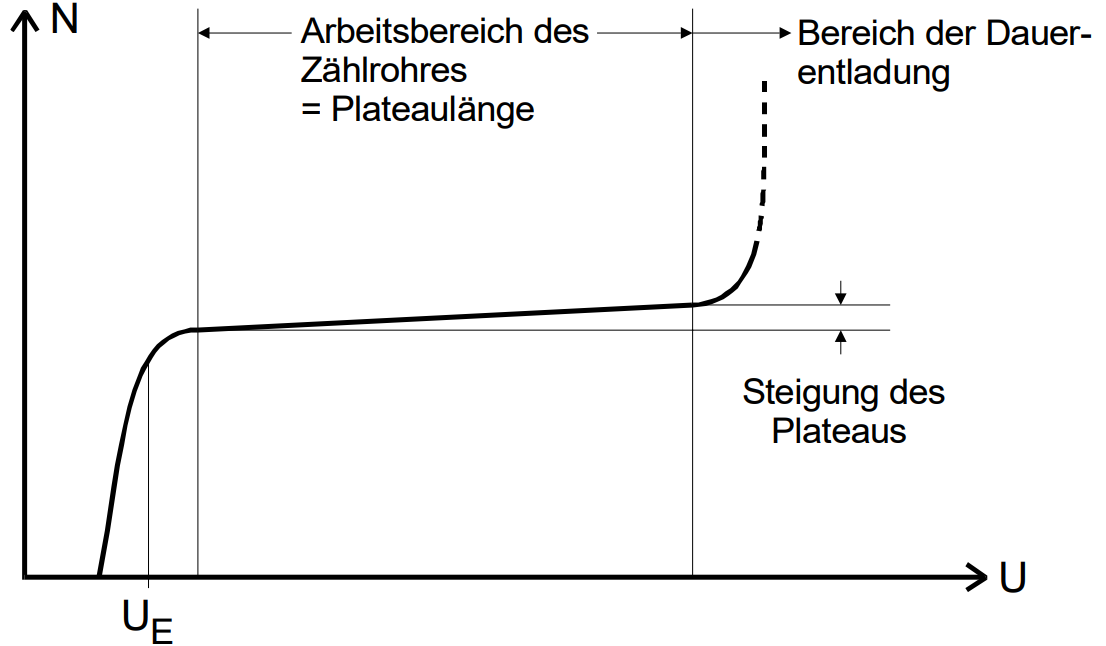
\includegraphics[width=\textwidth]{build/charakteristik.pdf}
  \caption{Auftragung der Zählrate gegen die Spannung und lineare Ausgleichsrechnung
  im Bereich des Plateaus.}
  \label{fig:plateau}
\end{figure}

Der Bereich des Plateaus befindet sich dabei zwischen den
beiden vertikalen grünen Linien. Mit den rot markierten Messwerten wird eine lineare
Ausgleichsrechnung der Form
\begin{equation}
  f(x)=ax+b
\end{equation}
durchgeführt. Die in blau eingezeichneten Messwerte werden für diese nicht mit
einbezogen. Es ergeben sich die Parameter
\begin{align*}
  a = (0{,}0361 \pm 0{,}0020)\, \frac{1}{\text{V\,s}} \,,\\
  b = (136{,}4 \pm 1{,}0)\,\frac{1}{\text{s}} \,.
\end{align*}
Die Steigung des Plateaus eines Zählrohres wird üblicherweise in $\%$ pro 100\,V
angegeben. Diese Angabe ist etwas irreführend, da die Steigung die Einheit
$\frac{1}{\text{V\,s}}$ besitzt. Wird sie dennoch in der üblichen Einheit angegeben,
so ergibt sich für die Steigung des Plateaus
\begin{equation*}
  a=(3{,}61 \pm 0{,}20) \symup{\frac{\%}{100V}} \,.  %Vielleicht noch mal mal 100???
\end{equation*}
Diese Einheit dient lediglich der Veranschaulichung. Sie soll verdeutlichen, um welchen
Faktor die Zählrate bei einer Zunahme der ans Zählrohr angelgten Spannung von 100\,V
steigt. 





Es soll nun die pro in das Zählrohr einfallende Teilchen freigesetzte Ladung
als Vielfaches der Elementarladung $e_0$ bestimmt werden. Dafür wird mithilfe von
Gleichung \eqref{eqn:ladung} zunächst die Ladungsmenge bestimmt. Die Ladungsmenge wird durch die
Elektronenladung $e_0$ dividiert, um die Anzahl der freigesetzten Elektronen
zu erhalten. Der Fehler ergibt sich dabei
gemäß der Gauß'schen Fehlerforpflanzung nach Gleichung \eqref{eqn:gaussfehler} zu
\begin{equation*}
  \sigma_{\symup{\Delta Q}}=\sqrt{\frac{I \Delta t}{N e_0}}=\sqrt{\frac{\Delta Q}{e_0}} \,.
\end{equation*}
Da $\frac{\Delta Q}{e_0}$ in der Größenordnung von $10^{10}$ und der Fehler in der
Größenordnung $10^{5}$, also vergleichsweise sehr gering ist, werden die
Werte im Folgenden als fehlerlos betrachtet. Daher wird auch auf das Einzeichnen von
Fehlerbalken verzichtet. Die berechneten Werte
befinden sich in Tabelle \ref{tab:messwerte}.
In Abbildung \ref{fig:ladung} ist die Anzahl der freigesetzten Elektronen
gegen die ans Zählrohr angelegte Spannung aufgetragen.

\begin{figure}
  \centering
  \includegraphics[width=\textwidth]{build/ladung.pdf}
  \caption{Auftragung der Anzahl der im Zählrohr freigesetzten Elektronen gegen die Spannung.}
  \label{fig:ladung}
\end{figure}

Der Verlauf der Messwerte sollte dem in Abbildung \ref{fig:nu} folgen. Zu Beginn ist
dieser Verlauf gut zu erkennen, ab Spannungen von etwa 400\,V folgen die Messwerte
jedoch einem annähernd linearen Verlauf. Laut der Theoriekurve sollte es hier
einen exponentiellen Anstieg geben.

\subsection{Bestimmung der Totzeit des Zählrohres}
\label{subsec:totzeit}
Die bei der Bestimmung der Totzeit mithilfe des Oszilloskops aufgenommenen Messwerte
befinden sich in Tabelle \ref{tab:totzeit_osz}. Diese werden gemäß den Gleichungen
\eqref{eqn:mean} und \eqref{eqn:std} gemittelt. So ergibt sich für die Totzeit
\begin{equation*}
  T_{\symup{Osz}}=(117\pm11)\,\text{µs}\,.
\end{equation*}

\begin{table}[htp]
	\begin{center}
    \caption{Vom Oszilloskop abgelesene Totzeiten für verschiedene Spannungen.}
    \label{tab:totzeit_osz}
		\begin{tabular}{cc}
		\toprule
			{$U/$V} & {$T/$µs} \\
			\midrule
      400 &  100    \\
      450 &  110    \\
      500 &  120    \\
      550 &  125    \\
      600 &  130    \\
		\bottomrule
		\end{tabular}
	\end{center}
\end{table}

Bei der Bestimmung der Totzeit mithilfe des Vergleichs der Zählraten der zwei
Proben wurden die in Tabelle \ref{tab:totzeit_exp} aufgeführten Werte gemessen.
Aus diesen Werten wird wie zuvor die Zählrate $Z$ berechnet. Gemessen wurde hier
bei einer Spannung von $U= 600\,$V.

\begin{table}[htp]
	\begin{center}
    \caption{Anzahl der Impulse der verschiedenen Proben und daraus berechnete Werte.}
    \label{tab:totzeit_exp}
		\begin{tabular}{ccc}
		\toprule
			& {$N$} & {$Z/$(1/s)} \\
      \midrule
      Strahler 1    &   12270 \pm 110  &  204,6 \pm 1,8   \\
      Strahler 2    &   13080 \pm 120  &  217,9 \pm 1,9   \\
      Strahler 1+2  &   24710 \pm 160  &  411,8 \pm 2,6   \\
		\bottomrule
		\end{tabular}
	\end{center}
\end{table}

Die Berechnung der Totzeit erfolgt gemäß Gleichung \eqref{eqn:zweiquellentotzeit}.
Der dabei entstehende Fehler ergibt sich mithilfe der Gauß'schen Fehlerfortpflanzung
nach Gleichung \eqref{eqn:gaussfehler} zu
\begin{center}
  $\sigma_T = \sqrt{\sigma_{\symup{N_1}}^{2} \left(\frac{1}{2 \symup{N_1} \symup{N_2}}
  - \frac{\symup{N_1} + \symup{N_2} - \symup{N_{1+2}}}{2 \symup{N_1}^{2} \symup{N_2}}\right)^{2}
  + \sigma_{\symup{N_2}}^{2} \left(\frac{1}{2 \symup{N_1} \symup{N_2}}
  - \frac{\symup{N_1} + \symup{N_2} - \symup{N_{1+2}}}{2 \symup{N_1} \symup{N_2}^{2}}\right)^{2}
  + \frac{\sigma_{\symup{N_{1+2}}}^{2}}{4 \symup{N_1}^{2} \symup{N_2}^{2}}} \,.$
\end{center}
Für die Totzeit ergibt sich damit bei dieser Methode
\begin{equation*}
  T_{\symup{ZQ}}= (120 \pm 40)µs \,.
\end{equation*}
